% fig_pinn_boundary.tex
% TR-46: PINN vs baseline accuracy in the k_ibr-alpha decision space
%
% Show the four protection zones in the (k_ibr, alpha) plane
% with PINN accuracy annotations

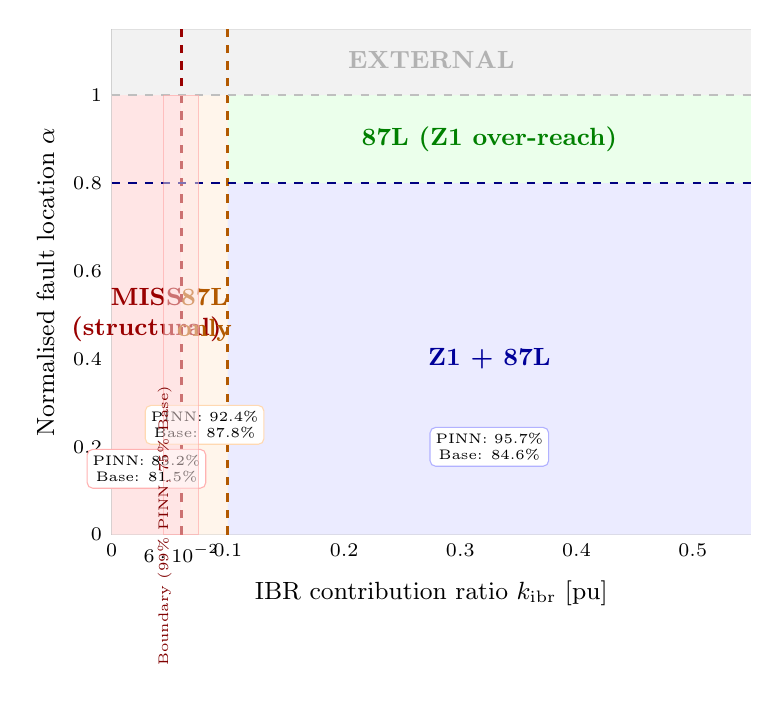
\begin{tikzpicture}
\begin{axis}[
  name         = bndax,
  width        = 0.80\textwidth,
  height       = 8.0cm,
  xlabel       = {IBR contribution ratio $k_\mathrm{ibr}$ [pu]},
  ylabel       = {Normalised fault location $\alpha$},
  xlabel style = {font=\small},
  ylabel style = {font=\small},
  xmin=0, xmax=0.55,
  ymin=0, ymax=1.15,
  xtick        = {0,0.06,0.10,0.20,0.30,0.40,0.50},
  ytick        = {0,0.2,0.4,0.6,0.8,1.0},
  xticklabel style={font=\scriptsize},
  yticklabel style={font=\scriptsize},
  tick style   = {draw=none},
  axis line style={gray!50},
  grid         = major,
  grid style   = {gray!10, dashed},
  clip=false,
]

%% Zone fills
% MISS zone: k < 0.06 (red-ish)
\addplot[red!15, fill=red!10, draw=none]
  coordinates {(0,0) (0.06,0) (0.06,1.0) (0,1.0)} \closedcycle;

% 87L-only zone: 0.06 ≤ k < 0.10
\addplot[orange!15, fill=orange!8, draw=none]
  coordinates {(0.06,0) (0.10,0) (0.10,1.0) (0.06,1.0)} \closedcycle;

% Z1 zone: k ≥ 0.10, alpha ≤ 0.80
\addplot[blue!15, fill=blue!8, draw=none]
  coordinates {(0.10,0) (0.55,0) (0.55,0.80) (0.10,0.80)} \closedcycle;

% 87L+Z1 zone: k ≥ 0.10, alpha > 0.80
\addplot[green!15, fill=green!8, draw=none]
  coordinates {(0.10,0.80) (0.55,0.80) (0.55,1.0) (0.10,1.0)} \closedcycle;

% EXT zone: alpha > 1.0
\addplot[gray!20, fill=gray!10, draw=none]
  coordinates {(0,1.0) (0.55,1.0) (0.55,1.15) (0,1.15)} \closedcycle;

%% Zone boundaries
\addplot[red!60!black, very thick, dashed]
  coordinates {(0.06,0) (0.06,1.15)};
\addplot[orange!70!black, very thick, dashed]
  coordinates {(0.10,0) (0.10,1.15)};
\addplot[blue!50!black, thick, dashed]
  coordinates {(0,0.80) (0.55,0.80)};
\addplot[gray!50, thick, dashed]
  coordinates {(0,1.0) (0.55,1.0)};

%% Zone labels
\node[red!60!black, font=\small\bfseries, align=center]
  at (axis cs:0.030, 0.50) {MISS\\(structural)};
\node[orange!70!black, font=\small\bfseries, align=center]
  at (axis cs:0.080, 0.50) {87L\\only};
\node[blue!60!black, font=\small\bfseries, align=center]
  at (axis cs:0.325, 0.40) {Z1 + 87L};
\node[green!50!black, font=\small\bfseries, align=center]
  at (axis cs:0.325, 0.90) {87L (Z1 over-reach)};
\node[gray!60, font=\small\bfseries]
  at (axis cs:0.275, 1.08) {EXTERNAL};

%% PINN accuracy annotations
\node[draw=blue!30, fill=white, rounded corners=2pt,
      font=\tiny, inner sep=2pt, align=center]
  at (axis cs:0.325, 0.20)
  {PINN: 95.7\%\\Base: 84.6\%};

\node[draw=orange!30, fill=white, rounded corners=2pt,
      font=\tiny, inner sep=2pt, align=center]
  at (axis cs:0.080, 0.25)
  {PINN: 92.4\%\\Base: 87.8\%};

\node[draw=red!30, fill=white, rounded corners=2pt,
      font=\tiny, inner sep=2pt, align=center]
  at (axis cs:0.030, 0.15)
  {PINN: 85.2\%\\Base: 81.5\%};

%% Boundary region highlight
\addplot[red!40, fill=red!10, opacity=0.5]
  coordinates {(0.045,0) (0.075,0) (0.075,1.0) (0.045,1.0)} \closedcycle;
\node[red!50!black, font=\tiny, rotate=90, anchor=south]
  at (axis cs:0.060, 0.02)
  {Boundary (99\% PINN, 75\% Base)};

\end{axis}
\end{tikzpicture}
